% Chapter Chapter 3 For Reproducible Research in R and RStudio
% Christopher Gandrud
% Created: 16/07/2012 05:45:03 pm CEST
% Updated: 16 January 2013




\chapter{Getting Started with R, RStudio, and knitr}\label{GettingStartedRKnitr}

If you have rarely or never used R before, the first section of this chapter gives you enough information to be able to get started and understand the R code I use in this book. For more detailed introductions on how to use R please refer to the resources I mentioned in Chapter \ref{Intro}. Experienced R users might want to skip the first section. In the second section I'll give a brief overview of RStudio. I highlight the key features of the main RStudio panel (what appears when you open RStudio) and some of its key features for reproducible research. Finally, I discuss the basics of the {\emph{knitr}} package, how to use it in R, and how it is integrated into RStudio.

%%%%%%%%%%%%% Using R
\section{Using R: the basics}

To get you started with reproducible research, we'll cover some very basic R syntax--the rules for talking to R. I cover key parts of R including:

\begin{itemize}
    \item objects \& assignment,
    \item component selection,
    \item functions and commands,
    \item arguments,
    \item the workspace and history,
    \item libraries.
\end{itemize}

Before discussing each of these in detail let's open R and look around.\footnote{Please see Chapter \ref{Intro} for instructions on how to install R.} When you open the R GUI program you should get a window that looks something like Figure \ref{RBlankMain}.\footnote{This figure and almost all screenshots in this book were taken on a computer using the Mac OS 10.8 operating system.} This window is the {\bf{R console}}\index{R!Console}. After the startup information--information about what version of R you are using, license details, and so on--you should see a {\tt{\textgreater}}. This prompt is where you enter R code.\footnote{If you are using a Unix-like\index{Unix} system such as Ubuntu\index{Ubuntu} or Mac OS 10\index{Mac}, you can also access R via an application called the Terminal\index{Terminal}. If you have installed R on your computer you can type {\tt{r}} into the Terminal and then the {\tt{Enter}} or {\tt{Return}} key. This will begin a new R session. You know if a new R session has started if you get the same startup information is printed in the Terminal window.} To run R code that you have typed after the prompt hit the {\tt{Enter}} or {\tt{Return}} key. Now that we have a new R session\index{R!session} open we can get started. 

\begin{figure}[th!]
    \caption{R Startup Console}
    \label{RBlankMain}
    \begin{center}
    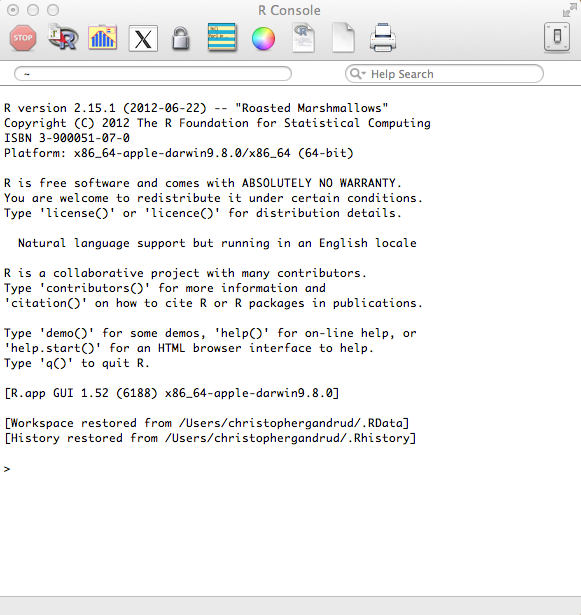
\includegraphics[scale=0.4]{Children/Chapter3/images3/BlankRConsole.png}
    \end{center}
\end{figure}

\subsection{Objects}\label{Objects}

If you've read a description of R before, you will probably have seen it referred to as an `object-oriented\index{object-oriented} language'.  What are objects? Objects are like the R language's nouns. They are things, like a vector of numbers, a data set, a word, a table of results from some analysis, and so on. Saying that R is `object-oriented' just means that R is focused on doing actions to objects. We will talk about the actions--commands and functions--later in this section.\footnote{Somewhat confusingly, commands and functions are themselves objects. In this Chapter I treat them as distinct from other object types.} For now let's create a few objects.

\paragraph{Numeric \& string objects}

Objects can have a number of different data types. Let's make two simple objects. The first is a numeric type object. The other is a character object. We can choose almost any name\label{ObjectNames} we want for our objects as long as it begins with an alphabetic character and does not contain spaces.\footnote{It is common for people to use either periods (\texttt{.}) or capital letters (referred to as CamelBack) to separate words in object names instead of using spaces. For example: {\emph{new.data}} or {\emph{NewData}} rather than {\emph{new data}}.} Let's call our numeric object {\emph{Number}}. It is a good idea to give each object a different name. Also make sure that object names are different from variable names. This will avoid many complications like accidentally overwriting an object or confusing R about what object or component you are referring to.

To put something into the object we use the assignment operator\index{R!assigmnent operator}\footnote{The assignment operator is sometimes also referred to as the `gets arrow'.}: {\tt{\textless -}}. Let's assign the number 10 to our {\emph{Number}} object.

\begin{knitrout}
\definecolor{shadecolor}{rgb}{0.969, 0.969, 0.969}\color{fgcolor}\begin{kframe}
\begin{alltt}
Number <- 10
\end{alltt}
\end{kframe}
\end{knitrout}


\noindent To see the contents of our object, type its name.

\begin{knitrout}
\definecolor{shadecolor}{rgb}{0.969, 0.969, 0.969}\color{fgcolor}\begin{kframe}
\begin{alltt}
Number
\end{alltt}
\begin{verbatim}
## [1] 10
\end{verbatim}
\end{kframe}
\end{knitrout}


\noindent Lets's briefly breakdown this output. \texttt{10} is clearly the contents of {\emph{Number}}. The double hash (\texttt{\#\#}) is included to tell you that this is output rather than R code.\footnote{The double hash is generated automatically by {\emph{knitr}}. It makes easier to copy and past code into R from a presentation document by {\emph{knitr}}.} If you type the commands in your R Console, you will not get the double hash in your output. Finally, \texttt{[1]} is the row number of the object that 10 is on. Clearly our object only has one row.   

Creating a character object is very similar. The only difference is that you enclose the character string (letters in a word for example) inside of single or double quotation marks (\verb|''|, or \verb|""|).\footnote{Single and double quotation marks are interchangable in R for this purpose. In this book I always use double quotes, except for \emph{knitr} code chunk options.} To create an object called \emph{Words} that contains the character string ``Hello World".\label{StringObject}

\begin{knitrout}
\definecolor{shadecolor}{rgb}{0.969, 0.969, 0.969}\color{fgcolor}\begin{kframe}
\begin{alltt}
Words <- \hlstring{"Hello World"}
\end{alltt}
\end{kframe}
\end{knitrout}


An object's type is important to keep in mind as it determines what we can do to it. For example, you cannot take the mean of a character object like the {\emph{Words}} object we created earlier:

\begin{knitrout}
\definecolor{shadecolor}{rgb}{0.969, 0.969, 0.969}\color{fgcolor}\begin{kframe}
\begin{alltt}
\hlfunctioncall{mean}(Words)
\end{alltt}


{\ttfamily\noindent\textcolor{warningcolor}{\#\# Warning: argument is not numeric or logical: returning NA}}\begin{verbatim}
## [1] NA
\end{verbatim}
\end{kframe}
\end{knitrout}


\noindent Trying to find the mean of our {\emph{Words}} object gave us a warning message and returned the value {\tt{NA}}\index{NA}: not applicable. You can also think of {\tt{NA}} as meaning missing. To find out what type of object you have use the {\tt{class}} command. For example:

\begin{knitrout}
\definecolor{shadecolor}{rgb}{0.969, 0.969, 0.969}\color{fgcolor}\begin{kframe}
\begin{alltt}
\hlfunctioncall{class}(Words)
\end{alltt}
\begin{verbatim}
## [1] "character"
\end{verbatim}
\end{kframe}
\end{knitrout}


\paragraph{Vector \& data frame objects}

So far we have only looked at objects with a single number or character string.\footnote{These might be called scalar objects, though in R scalars are just vectors with a length of 1.} Clearly we often want to use objects that have many strings and numbers. In R these are usually data frame\index{data frame} type objects and are roughly equivalent the data structures you would be familiar with from using a program such as Microsoft Excel. We will be using data frames extensively throughout the book. Before looking at data frames it is useful to first look at the simpler objects that make up data frames. These are called vectors. Vectors are R's ``workhorse" \cite[]{Matloff2011}. Knowing how to use vectors\index{vector} will be especially helpful when you clean up raw data in Chapter \ref{DataClean} and make tables in Chapter \ref{TablesChapter}.\footnote{If you want information about other types of R objects such as lists\index{list} and matrices\index{matrix}, Chapter 1 of Norman Matloff's \citeyearpar{Matloff2011} book is a really good place to look.} \\[0.25cm]

\noindent {\bf{Vectors}} \\[0.25cm] Vectors are the ``fundamental data type" in R \cite[]{Matloff2011}. They are simply an ordered group of numbers, character strings, and so on.\footnote{In a vector every member of the group must be of the same type. If you want an ordered group of values with different types you can use lists.} It may be useful to think of basically all R objects as composed of vectors. For example, data frames are basically multiple vectors of the same length--i.e. they have the same number of rows--attached together to form columns. 

Let's create a simple numeric vector containing the numbers 2.8, 2, and 14.8. To do this we will use the \texttt{c} (concatenate)\index{concatenate} function:

\begin{knitrout}
\definecolor{shadecolor}{rgb}{0.969, 0.969, 0.969}\color{fgcolor}\begin{kframe}
\begin{alltt}
NumericVect <- \hlfunctioncall{c}(2.8, 2, 14.8)

\hlcomment{# Show NumericVect's contents}
NumericVect
\end{alltt}
\begin{verbatim}
## [1]  2.8  2.0 14.8
\end{verbatim}
\end{kframe}
\end{knitrout}


Vectors of character strings are created in a similar way. The only major difference is that each character string is enclosed in quotation marks like this:

\begin{knitrout}
\definecolor{shadecolor}{rgb}{0.969, 0.969, 0.969}\color{fgcolor}\begin{kframe}
\begin{alltt}
CharacterVect <- \hlfunctioncall{c}(\hlstring{"Albania"}, \hlstring{"Botswana"}, \hlstring{"Cambodia"})

\hlcomment{# Show CharacterVect's contents}
CharacterVect
\end{alltt}
\begin{verbatim}
## [1] "Albania"  "Botswana" "Cambodia"
\end{verbatim}
\end{kframe}
\end{knitrout}


To give you a preview of what we are going to do when we start working with real data sets, lets combine the two vectors {\emph{NumericVect}} and {\emph{CharacterVect}} into a new object with the \texttt{cbind}\index{R command!cbind} function. This function binds the two vectors together side-by-side as columns.\footnote{If you want to combine objects as if they were rows of the same column(s) use the \texttt{rbind}\index{rbind} function.}\label{cbind}

\begin{knitrout}
\definecolor{shadecolor}{rgb}{0.969, 0.969, 0.969}\color{fgcolor}\begin{kframe}
\begin{alltt}
StringNumObject <- \hlfunctioncall{cbind}(CharacterVect, NumericVect)

\hlcomment{# Show StringNumObject's contents}
StringNumObject
\end{alltt}
\begin{verbatim}
##      CharacterVect NumericVect
## [1,] "Albania"     "2.8"      
## [2,] "Botswana"    "2"        
## [3,] "Cambodia"    "14.8"
\end{verbatim}
\end{kframe}
\end{knitrout}


\noindent By binding these two objects together we've created a new matrix\index{matrix} object.\footnote{Matrices are vectors with columns as well as rows.} You can see that the numbers in the {\emph{NumericVect}} column are between quotation marks. Matrices, like vectors can only have one data type. \\[0.25cm]

\noindent {\bf{Data frames}}

If we want to have an object with rows and columns and allow the columns to contain data with different types, we need to use data frames\index{data frame}. Let's use the \texttt{data.frame}\index{R command!data.frame} command to combine the {\emph{NumericVect}} and {\emph{CharacterVect}} objects.\label{data.frame}

\begin{knitrout}
\definecolor{shadecolor}{rgb}{0.969, 0.969, 0.969}\color{fgcolor}\begin{kframe}
\begin{alltt}
StringNumObject <- \hlfunctioncall{data.frame}(CharacterVect, NumericVect)

\hlcomment{# Display contents of StringNumObject data frame}
StringNumObject
\end{alltt}
\begin{verbatim}
##   CharacterVect NumericVect
## 1       Albania         2.8
## 2      Botswana         2.0
## 3      Cambodia        14.8
\end{verbatim}
\end{kframe}
\end{knitrout}


\noindent There are a few important things to notice in this output. The first is that because we used the same name for the data frame object as the previous matrix object, R deleted the matrix object and replaced it with the data frame. This is something to keep in mind when you are creating new objects. In general it is a better idea to assign elements to new objects rather than overwriting old ones. This will help avoid accidentally using an object you had not intended to. It also allows you to more easily change previously run source code.

You can see the data frame's names\index{R command!names} attribute.\footnote{Matrices can also have a names attribute.} It is the column names. You can use the \texttt{names} command to see any data frame's names:\footnote{You can also use \texttt{names} to assign names for the entire data frame. For example, \texttt{names(StringNumObject) <- c("Variable1", "Variable2")}}

\begin{knitrout}
\definecolor{shadecolor}{rgb}{0.969, 0.969, 0.969}\color{fgcolor}\begin{kframe}
\begin{alltt}
\hlfunctioncall{names}(StringNumObject)
\end{alltt}
\begin{verbatim}
## [1] "CharacterVect" "NumericVect"
\end{verbatim}
\end{kframe}
\end{knitrout}


You will also notice that the first column of the data set has no name and is a series of numbers. This is the row.names attribute.\index{row.names} Unlike with matrices, data frame rows can be given any name as long as they are unique. We can use the \texttt{row.names} command to set the row names from a vector. For example,

\begin{knitrout}
\definecolor{shadecolor}{rgb}{0.969, 0.969, 0.969}\color{fgcolor}\begin{kframe}
\begin{alltt}
\hlcomment{# Reassign row.names}
\hlfunctioncall{row.names}(StringNumObject) <- \hlfunctioncall{c}(\hlstring{"First"}, \hlstring{"Second"}, \hlstring{"Third"})

\hlcomment{# Display new row.names}
\hlfunctioncall{row.names}(StringNumObject)
\end{alltt}
\begin{verbatim}
## [1] "First"  "Second" "Third"
\end{verbatim}
\end{kframe}
\end{knitrout}


You can see in this example how the \texttt{row.names} command can also be used to see the row names.\footnote{Note that this is really only useful for data frames with few rows.} The row.names attribute does not behave like a regular data frame column. You cannot, for example include it as a variable in a regression. You can use the \emph{row.names} command to assign the row.names values to a regular column (for an example see page \pageref{RowNamesTidy}). 

You will notice in the output for \emph{StringNumObject} that the strings in the \textbf{CharacterVect} column are no longer in quotation marks. This does not mean that they are somehow now numeric data. To prove this try to find the mean of \textbf{CharacterVect} by running it through the \texttt{mean}\index{R command!mean} command:

\begin{knitrout}
\definecolor{shadecolor}{rgb}{0.969, 0.969, 0.969}\color{fgcolor}\begin{kframe}
\begin{alltt}
\hlfunctioncall{mean}(StringNumObject$ChacterVect)
\end{alltt}


{\ttfamily\noindent\textcolor{warningcolor}{\#\# Warning: argument is not numeric or logical: returning NA}}\begin{verbatim}
## [1] NA
\end{verbatim}
\end{kframe}
\end{knitrout}


\subsection{Component Selection}

The last bit of code will probably be confusing. Why do we have a dollar sign (\texttt{\$}) in between the name of our data frame object and the \textbf{CharcterVect}? The dollar sign is called the component selector.\index{component selector}\index{R!\$, component selector}\footnote{It's also sometimes called the element name operator.} It basically extracts a part--component--of an object. In the previous example it extracted the \textbf{CharacterVect} column from the {\emph{StringNumObject}} and fed it to the \texttt{mean} command, which tried (in this case unsuccessfully) to find its mean.

We can of course use the component selector to create new objects with parts of other objects. Imagine that we have the {\emph{StringNumObject}} and want an object with only the information in the numbers column. Let's use the following code:

\begin{knitrout}
\definecolor{shadecolor}{rgb}{0.969, 0.969, 0.969}\color{fgcolor}\begin{kframe}
\begin{alltt}
NewNumeric <- StringNumObject$NumericVect

\hlcomment{# Display contents of NewNumeric}
NewNumeric
\end{alltt}
\begin{verbatim}
## [1]  2.8  2.0 14.8
\end{verbatim}
\end{kframe}
\end{knitrout}


\noindent Knowing how to use the component selector will be especially useful when we discuss making tables for presentation documents in Chapter \ref{TablesChapter}.

Using the component selector can lead to long repetitive code. You have to write the object name, a dollar sign, and the component name every time you want to select a component. You can streamline your code by using commands such as \texttt{attach}\index{R command!attach} and \texttt{with}\index{R command!with}. 

The \texttt{attach} command attaches a database to R's search path,\index{R!search path} i.e. it searchers the database for variables you specify. You don't need to use the component selector to tell R to look in a particular data frame after you have attached it. For example:

\begin{knitrout}
\definecolor{shadecolor}{rgb}{0.969, 0.969, 0.969}\color{fgcolor}\begin{kframe}
\begin{alltt}
\hlcomment{# Attach StringNumObject to search path}
\hlfunctioncall{attach}(StringNumObject)
\end{alltt}
\begin{verbatim}
## The following object(s) are masked _by_ '.GlobalEnv':
## 
##     CharacterVect, NumericVect
## The following object(s) are masked from 'StringNumObject (position 3)':
## 
##     CharacterVect, NumericVect
\end{verbatim}
\begin{alltt}

\hlcomment{# Display contents of NumericVect}
NumericVect
\end{alltt}
\begin{verbatim}
## [1]  2.8  2.0 14.8
\end{verbatim}
\begin{alltt}

\hlcomment{# Detach StringNumObject}
\hlfunctioncall{detach}(StringNumObject)
\end{alltt}
\end{kframe}
\end{knitrout}


\noindent It is a good idea to \texttt{detach}\index{R command!detach} a data frame after you are done using it, to avoid confusing R. 

Similarly you can use \texttt{with} to run a command using a particular database. For example, we can find the mean of \emph{NumericVect} \texttt{with} the \emph{StringNumObject} data frame:





























































